\documentclass[10pt,twocolumn]{IEEEtran}

\usepackage[linesnumbered,lined,boxed,commentsnumbered, noend, noline]{algorithm2e}
\usepackage{graphicx}
\usepackage{xcolor}
\usepackage{soul}

\newcommand{\hlc}[2][yellow]{{%
    \colorlet{foo}{#1}%
    \sethlcolor{foo}\hl{#2}}%
}

\title{Analyzing Algorithmic Patterns Based on Real Coding Interview Questions}
\author{Ian Dempsey}
%\hlc[cyan!50]{_____} -> put in the stuff to be highlighted inside the {}
%cite{___} ->put in the bibtex key for the specific source.
%\label{sec: | fig: | } -> use to give something a specific label. This allows it to be referenced later
%\ref{___} -> to refernce a previously labeled area
\begin{document}

\maketitle
\pagenumbering{gobble}
\newpage
\pagenumbering{arabic}
\section{Abstract}
This is my abstract. It is empty for now. Fill in later
\section{Introduction}
\label{sec:intro}
\par
Nowadays interviews for jobs in the I.T industry are becoming more complex and demanding on the applicant. As this section of the working industry is usually quite technical, it is quite common for the applicants to have to perform some form of technical test. These tests normally involve a question or two that are based on a wide variety of topics in programming. These questions in particular are used to test potential employees on whether they have strong analytical and critical assessment skills. The technical tests also allow the employer to see how many standard algorithms the candidate knows and is able to use. However, it is difficult to master all of the different types of algorithms and their intricacies. 
\par The purpose of this paper is to study the relationship between the classical and well known algorithms, and the interview questions which are commonly asked.  This paper aims to give guidance to people who want to study the interview questions, but learn a core set of common ideas which will help them solve multiple problems. This would therefore allow them to save time as they prepare for the interview.
\par In this paper we present a comprehensive report summarising the similarities between interview questions and standard algorithms taught in any programming course. This distinguishes our work from interview preparation books which focus on the problem solving skills, simply showing the reader a solution to a single problem, and not reinforcing material they would already be familiar with. This paper's goal is to show people that understanding the fundamentals of several common algorithms, will allow them to be able to solve a wide array of problems. It is also the purpose of this paper that a beginner at programming or a fresh graduate can use this paper as guidance to show them how much time is needed for preparatory work before they have the interview.  
  %The questions themselves have a wide range of difficulty, from easier ones which focus on in basics of programming- e.g., array indexing, sorting algorithms, up to harder questions which really push candidates- e.g., dynamic programming, graphs. This area of interviewing is known as \textit{whiteboarding}, and has become quite common, it has led to some books being published which compile together numerous questions which are popular for interviewers to ask\cite{mcdowell2015cracking}.The focus in this paper is not the ability to solve as many quetions as possible to give to the applicants to study, but to try and discover patterns in problems which are similar, and then classify these patterns based off of pre-established patterns that candidates would be used to. This classification will then be able to help applicants and fellow programmers to learn how to see the patterns in problems quicker and be able to apply them to multiple problems, where they need only alter specific areas of code to solve the target problem. %
\section{Technical Background}
\par Nowadays there are a lot of online repositories for interview questions and interview related material in general. Websites such as hackerrank.com , glassdoor.ie, geeksforgeeks.org ,and leetcode.com all offer information on what questions are common during interviews for different companies. They also offer ways to test potential solutions to some of the given questions. 
\par For this paper we chose to use leetcode.com\cite{leet1}, as this website comes with a huge amount of online material that is generally taken from previously asked interview questions. Companies also use sites just like leetcode when they are building up a question bank to ask candidates. This was important in our decision for the repository, as it meant we were using a platform which was regularly updated. LeetCode itself also has some built-in features which really appealed to us. The website has an online discussion forum for each question, allowing the community to discuss solutions, issues and the questions themselves. LeetCode also host their own weekly coding competitions, which allows users to get even more experience and confidence in coding problems. One of the main features which this online judge website has in comparison to the others is a section for a user to perform a mock interview. This mock interview is under the time constraint of a normal real world interview, this was a big attraction for us in choosing our online judge. The online editor that is used by leetcode also allows a user to select from a multitude of programming languages, as shown in figure \ref{fig:langUI} below. For the purpose of this paper the language that was chosen was java. The reason for this is because it is a language most people learn first. However, any choice of programming language would be just as acceptable, as we present pseudocode throughout the paper which can be used by any major programming language.  
\par The user interface of LeetCode is also very simple to use. The main page which lists all of the problems offers users the option to filter questions by difficulty, which company has asked it before, what area the questions focuses on and much more. As seen in figure \ref{fig:homepage}, we have chosen to focus on questions which are tagged as being related to trees. 
\begin{figure}[h]
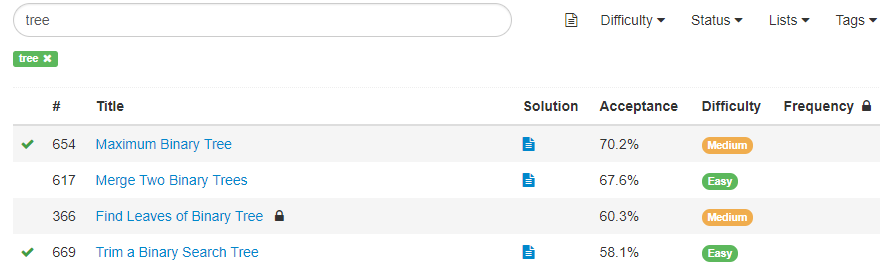
\includegraphics[width=0.5\textwidth]{homepageUI.png}
\caption{Homepage}
\label{fig:homepage}
\end{figure}

A user simply chooses the question which they wish to attempt, and is promptly brought to the problem's specific screen, as seen in figure \ref{fig:problemPage}. On this screen there is a general description of the problem and a few examples for more clarification. This page also contains the online editor that the user will use to attempt the problem. The online editor is quick and easy to understand, and as stated has a variety of options for the user to choose from. 
\begin{figure}[h]
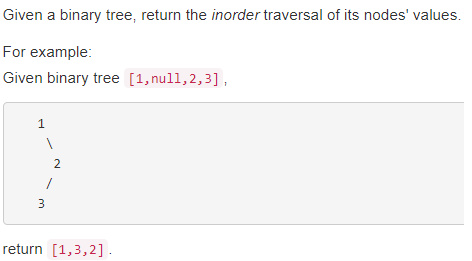
\includegraphics[width=0.5\textwidth]{problemPage.png}
\caption{Problem Specific Page}
\label{fig:problemPage}
\end{figure}

\begin{figure}[h]
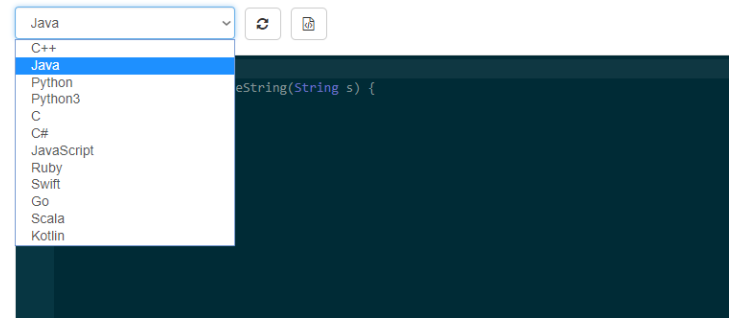
\includegraphics[width=0.5\textwidth]{languageUI.png}
\caption{Online editor with options displayed}
\label{fig:langUI}
\end{figure}   
The user will attempt to solve the problem they have selected and they will then want to submit their answer and see if it was correct, they perform this by clicking the submit solution button underneath the editor. Leetcode allows a user to sumbit their code and be informed almost instantly if they are correct or not. There are two possible outcomes once the user clicks the submit button. Either it is accepted and leetcode returns an accepted result with suggestions for the next question a user could attempt, shown in figure \ref{fig:accepted}, or their answer failed a certain testcase or even their code failed to compile and run, shown in figure \ref{fig:fail}. In the case of failure, leetcode will report where an error is in the code by referencing the line.  
\begin{figure}[h]
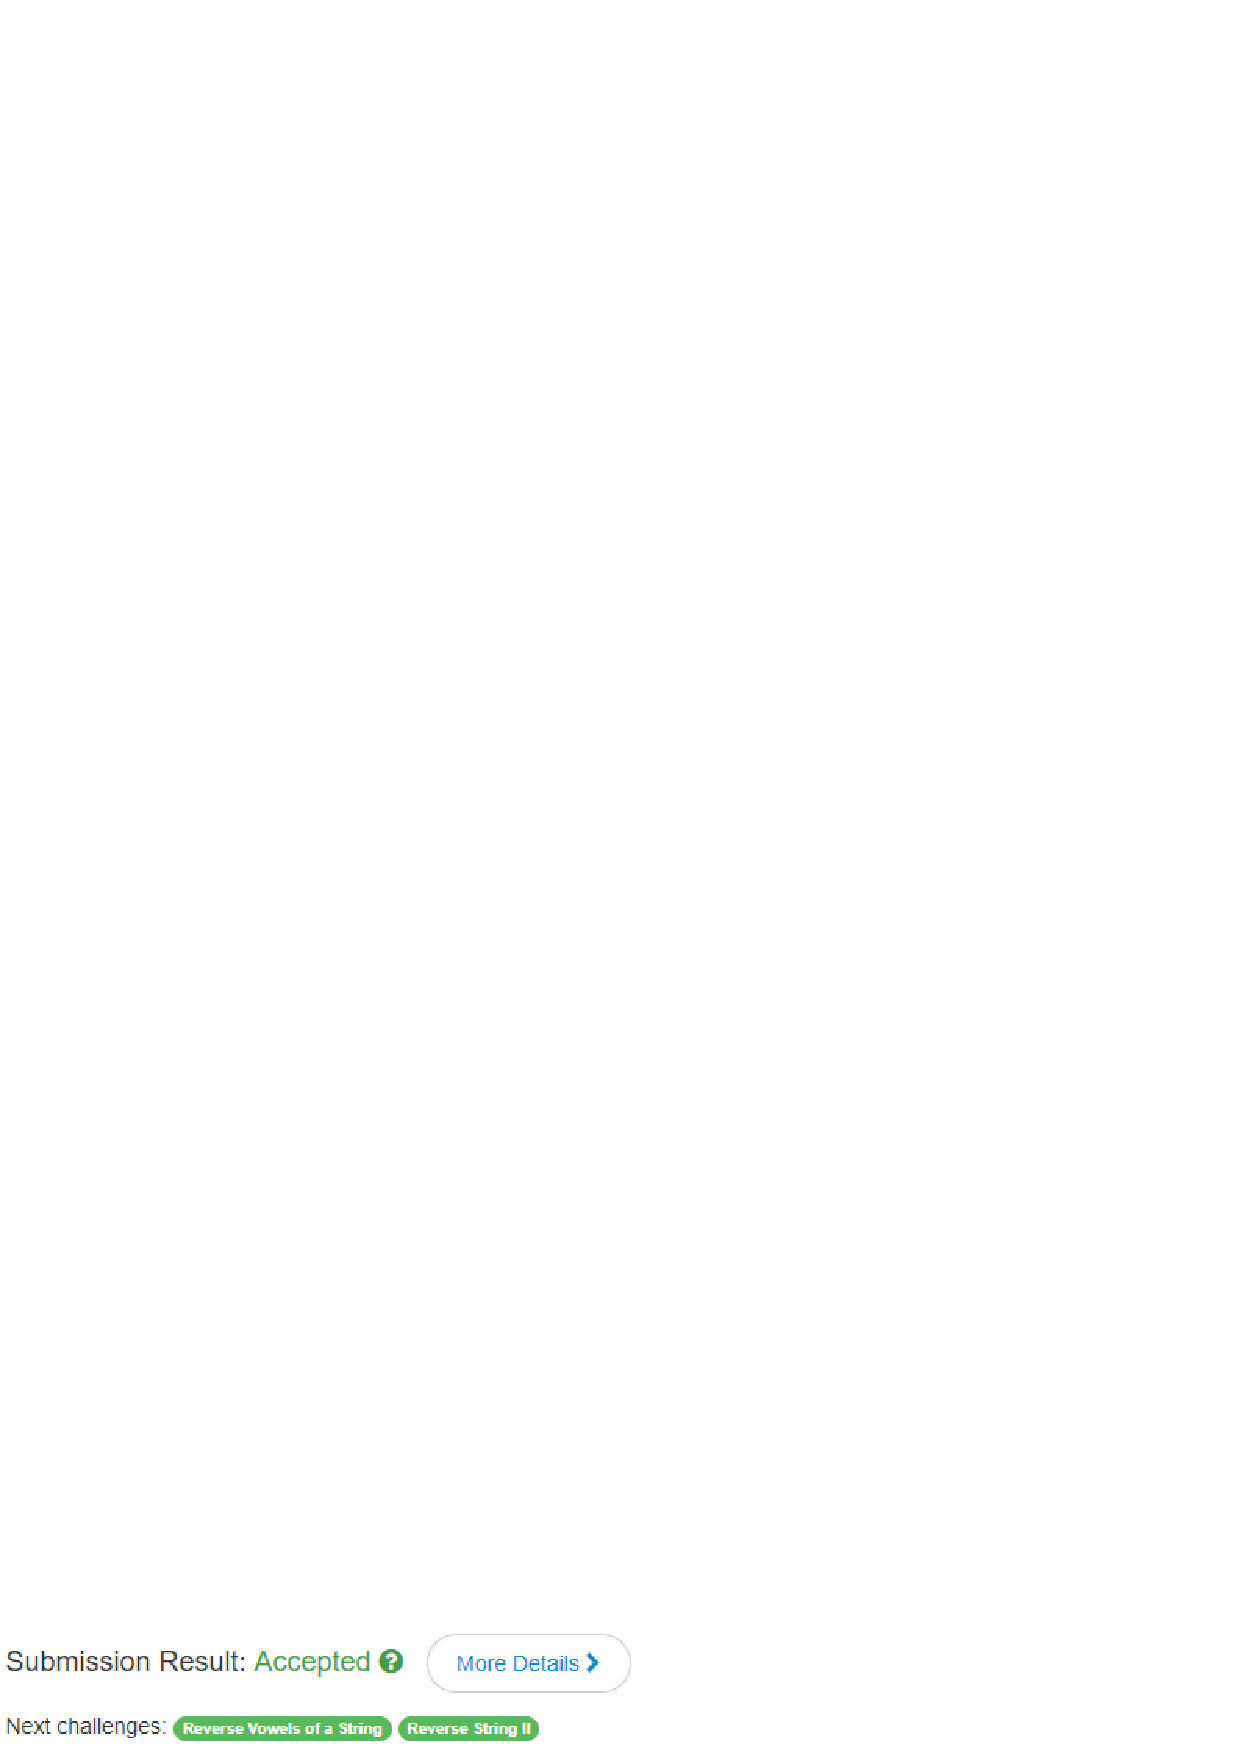
\includegraphics[width=0.5\textwidth]{accepted.png}
\caption{User solution passes all testcases}
\label{fig:accepted}
\end{figure}  
\begin{figure}[h]
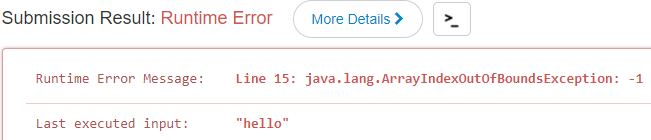
\includegraphics[width=0.5\textwidth]{failure.png}
\caption{User solution failing submission}
\label{fig:fail}
\end{figure}    

\section{Problem Statement}
In order to fulfill the goal of this paper, we will answer the following research questions:
\begin{enumerate}
\item What algorithms to choose, and what categories do these algorithms fall under. 
\item How do these algorithms relate to the classic algorithms and how similar are they.
\item How easy is it for a person to indentify the pattern of the algorithm.
\end{enumerate}
\section{General Patterns for Analysis}
\subsection{Palindrome}
Palindromes are extremely useful for searching algorithms, as Palindromes are meant to be the same in both directions, one can easily discover if the input is an actual palindrome. This is helpful for searching because one can search and find the odd character out, or the unique piece of data in some text. This style of algorithm is also space efficient, they normally have a space analysis of O(n/2) as the algorithm works over two elements of the input at a time. The basic approach of a Palindrome algorithm is to work inwards with both pointers starting at either end of the input and constantly moving towards one another and comparing if the elements are the same.\\  
The following description is a general algorithm for solving the palindrome problem which is a common problem in Java and other languages. This approach can be used to solve numerous other problems by altering the inside of the loop.
Pseudocode:
\IncMargin{1em}
\begin{algorithm}
	\SetAlgoLined
	\KwData{Given input of characters, S}
	\KwResult{Boolean}
	initialization\;
	$leftIndex  \longleftarrow $S[0]\;
	$rightIndex \longleftarrow $S.length-1\;
	\While{leftIndex $<$ rightIndex}{
	
	compare leftIndex with rightIndex\;
	\If{leftIndex !=rightIndex}{
		return false\;
	}
	 leftIndex++\;
	rightIndex++\;
}
return true\;
\caption{The Palindrome Algorithm}
\end{algorithm}\DecMargin{1em}

Whilst studying and working on this project, I have answered a number of questions from Leetcode.com which I was able to solve using an altered version of the above Palindrome pattern. Leetcode question 1 TwoSum is one example. This question is described as: \textit{Given an array of integers, return indices of the two numbers such that they add up to a specific target. You may assume that each input would have exactly one solution, and you may not use the same element twice.} The following pseudocode is my answer to this question. In it I have taken the basic idea of the Palindrome algorithm of having two pointers used for looking through the input data, but I have altered the way these two pointers behave.In this pseudocode I have highlighted any differences in blue.
\IncMargin{1em}
\begin{algorithm}
	\SetAlgoLined
	\KwData{Array of integers nums, target S}
	\KwResult{Indices i,j}
	$leftIndex  \longleftarrow $S[0]\;
	$rightIndex \longleftarrow $S.length-1\;
	\While{leftIndex $<$ rightIndex}{
	\hlc[cyan!50]{Sort the input array nums\;}\\
	\uIf{\hlc[cyan!50]{nums[leftIndex]+nums[rightIndex] $>$ S}}{
		\hlc[cyan!50]{rightIndex$--$\;}
	}\uElseIf{\hlc[cyan!50]{nums[leftIndex]+nums[rightIndex]$<$S}}{
		\hlc[cyan!50]{leftIndex++\;}
	}\Else{
		\hlc[cyan!50]{return leftIndex, rightIndex\;}
	}
     }return 0\;
\caption{LeetCode Q1 TwoSum}
\end{algorithm}\DecMargin{1em}\\
As can be seen from the above answer, the main differences are the conditionals inside the while loop. Instead of the normal approach of a Palindrome where one checks if the two elemts are equal, and if so moves the two pointers are moved at the same time towards eachother, I have changed the condisitionals such that instead of moving both of these pointers together at the same time, I only ever move one pointer at a time. Depending on the result of adding the two current elements at each pointer together. If the total from adding the two integers together was greater than the target sum, then I knew that I had to move the right-pointer left once, as this would allow me to have a smaller sum and potentially the correct sum. If on the other hand the sum was smaller than the total, I would only move the left-pointer right once and add the two elements and get a new result. This process was repeated until the target sum was found, or until the two pointers crossed which meant the target was not found.
\subsection{Merge Sort}
Merge Sort is a very powerful algorithm. It is more efficient than most styles of insertion, with a time analysis of $O(n * log_{n})$, whereas insertion is $O(n^2)$. The idea of merge sort is to divide an array or some input in half and then sort each half before joining it back together. They do not have to be the same size which is useful.  \\
Merge Sort uses the idea of divide and conquer, this means the list to be sorted should be divided up into equal parts first, then these new smaller parts should be sorted individually first before recreating the full list.
Pseudocode:
\IncMargin{1em}
\begin{algorithm}
	\SetAlgoLined
	\KwData{List of unsorted data}
	\KwResult{Sorted List}
 	\eIf{ length of A is 1}{ return 1}
  	{Split A into two halves , L and R. Repeat until size of part =1\\
  	Sort each part individually \\
  	Merge with another subdivided section into B, the sorted list\\ 
  	Return B, the sorted structure}
\caption{The Merge Sort Algorithm through Recursion}
\end{algorithm}\DecMargin{1em}

\subsection{Graphs}
Graphs are common in our lives. News media use them to help us visualize certain statistics. Though these are not the graphs that are studied by Computer Scientists. Graphs studied by Computer Scientists are usually based on the tree structure, and the relationships among data elements. A tree is just one of the special types of graphs that can be studied, where the parent-child relationship is used to organise data. In this section I have focused on the Tree Abstract Data Type, Breadth-First Traversal, Depth-First Traversal and Graphs in general. \\
\subsubsection{Trees}
Trees are one of the most powerful styles of data structures for processing data, this is because they allow rapid searching and fast insetion/deletion of a node. Trees are made up of nodes, these are Objects which hold some data and have a key. This key allows one to determine where this node should be in the tree. The important distinction here with these nodes in comparison to other nodes used in various data structures, is that these nodes contain references to children instead of just the next Link. Each node has exactly one parent, but can have many children.A Binary Tree is a special type of tree, this is a tree which has between 0 and 2 children. The first node in a tree is the Root, and it is possible to traverse to any node in the tree from this node.
With trees the main function is traversal. There are three basic styles of traversal: inorder, preorder and postorder. Inorder visits every Node in ascending order based on their key values. Preorder is where the root is visited first, followed by it's left subtree and then it's right subtree. Finally, postorder is where the left subtree is followed by the right subtree and then the root. \\
The following is an example of how one might search for a particular Node in a Tree.\\
Pseudocode:
\IncMargin{1em}
\begin{algorithm}
	\SetAlgoLined
	\KwData{Given a key to search for}
	\KwResult{The desired Node, or null}
	initialization\;
	$Node current \longleftarrow$root\;
	\While{current.data is not key}{
		\If{current is null}{return null\;}
		\eIf{current.data $>$ key}{
			move left on the tree\;
		}{
		move right on the tree\;
		}
	}
return current\;
\caption{Finding a specific Node in a tree based on the key}
\end{algorithm}\DecMargin{1em}
\\
\IncMargin{1em}
\begin{algorithm}
	\SetAlgoLined
	\SetKwFunction{postOrder}{postOrder}
	\Indm\postOrder{$Node localRoot$}
	%\KwData{Node localRoot}
	%\KwResult{Print out in PostOrder}
	\\
		\If{localRoot $!=$ null}{
		\postOrder(localRoot leftChild)\\
		\postOrder(localRoot rightChild)\\
		Print(localRoot data)\;}	
\caption{Basic Tree Traversal using PostOrder Traversal}
\end{algorithm}\DecMargin{1em}
\\
Leetcode question 104, \textit{Maximum Depth of Binary Tree}, is an example of a problem where I used the basic tree traversal styles to solve the question.The problem description is given as: \textit{Given a binary tree, find its maximum depth.The maximum depth is the number of nodes along the longest path from the root node down to the farthest leaf node.} In this algorithm I used postorder traversal. Pseudocode can be found in Algorithm 6 of this paper.\\
\IncMargin{1em}
\begin{algorithm}
	\SetKwFunction{maxDepth}{maxDepth}
	\Indm\maxDepth{$TreeNode  localRoot$}\\
	\SetAlgoLined
	%\KwData{Node localRoot}
	%\KwResult{Print out in PostOrder}
		\If{\hlc[cyan!50]{localRoot $==$ null}}{\hlc[cyan!50]{ return 0\;}}
		\hlc[cyan!50]{int ldepth $=$}\maxDepth(localRoot leftChild)\;
		\hlc[cyan!50]{int rdepth $=$}\maxDepth(localRoot rightChild)\;
		\If{\hlc[cyan!50]{ldepth $>$ rdepth}}{
		\hlc[cyan!50]{return ldepth+1}
		}\Else{\hlc[cyan!50]{return rdepth+1}}
\caption{Leetcode Q104 Max. Depth of Binary Tree}
\end{algorithm}\DecMargin{1em}
\\
As highlighted above, the key diference is inside the if statement. I have changed the conditional itself as it is the base case to stop the recursive execution. I have created a variable \textit{ldepth} which is the total depth of the left subtree. This is a recursive call on the leftChild of the current node. Line 4 will execute until it can't go left anymore, if it reaches null it will try to go right once, and then return going left. This is repeted until both calls return null. It then will go back all the way up until we reach the first call to go left, and set this summation of steps to ldepth. It then performs this same process but on the right subtree of the current node(which is the original node given), and set it to the variable \textit{rdepth}. Finally there is a conditional checking if ldepth is greater than rdepth. If so it returns ldepth+1,or it returns rdepth+1. This+1 is required as I need to take into account the root node's level, if I didn't take this into account my answer would always be one less than the actual depth of the tree. The major similarities between the postorder algorithm and this solution is the way I went down the left subtree first, then the right subtree and finally to take into account the root I added one to the height. This particular way of traversing the tree, left-right-root, is exactly how postorder traversal is performed.
\\
\subsubsection{Breadth-First Traversal}
This is a special way to visit the nodes in a tree, the ordering in this traversal pattern is to visit the root node, then move onto the children of the root node, printing each child in turn. It then will repeat this for each child of these nodes.Figure 1 shows the nodes in numerical order of visitation when using Breadth-First Traversal. \\
\begin{figure}[h]
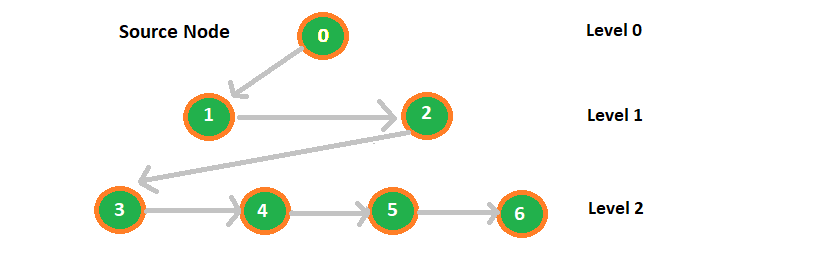
\includegraphics[width=0.6\textwidth]{bfs.png}
\caption{Breadth-First Traversal}
\end{figure}
 \\
\subsubsection{Depth-First Traversal}
This is a second way of visiting nodes in a tree. This pattern involves starting at the root node, then going to the left most child, then repeating this movement until the traversal reaches a leaf node (a node which has no children), then it will move back up one node and try to visit the next child node of this current node. It repeats this until the traversal finds no univisited node. Figure 2 shows the nodes in numerical order of visitation when using Depth-First Traversal. 
\begin{figure}[h]
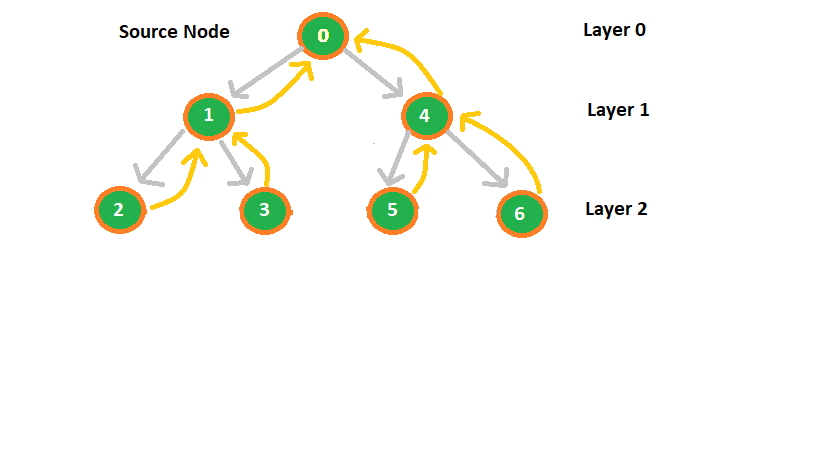
\includegraphics[width=0.6\textwidth]{dfs.png}
\caption{Depth-First Traversal}
\end{figure}

\section{The questions chosen}
I based all of my questions off of the six-hundred or so that were available on www.leetcode.com\cite{leet1}. To shrink the question pool that I was choosing from I would try to pick the quesitons which were under the filter of Top Interview Questions. I did pick questions which were not listed under this filter, as I felt that solving some questions from outside of this restriction allowed me to get a more diverse seletion of questions. Also the questions were tagged by the user base of the site. Meaning that some of the questions which were not listed as being interview related, could have been asked in one, and vice versa. This does lead to the issue of having faith in the honesty of the community on the site.  

\section{Problems with the questions}
Whilst working on the numerous questions that I have solved on leetcode.com, I did come across issues which related to the questions themselves. These problems stemmed from the questions being worded strangely, or the example given for the solution was not explicitly clear in the way the question worked. These were just some of the issues which occurred whilst attempting to solve the problems. An example of such an issue is leetcode question 654. Maximum Binary Tree. This question's problem was easy to understand:
\\ \textit {Given an integer array with no duplicates. A maximum tree building on this array is defined as follow:
\begin{enumerate}
\item The root is the maximum number in the array.
\item The left subtree is the maximum tree constructed from left part subarray divided by the maximum number.
\item The right subtree is the maximum tree constructed from right part subarray divided by the maximum number.
\end{enumerate}
Construct the maximum tree by the given array and output the root node of this tree.}\\
The issue which I personally came across was when I tried to understand the way the left and right subtree should be structured. The description for them was not clear to me, as I was unsure what was meant by $''$left part subarray divided by the maximum number$''$. I then took a look at the provided example.
\begin{figure}[h]
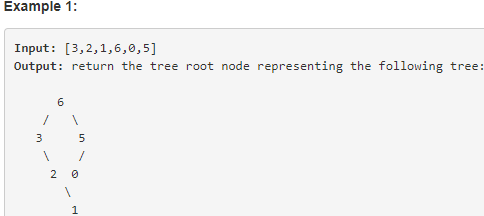
\includegraphics[width=0.6\textwidth]{example654.png}
\caption{Q654 Given Example}
\end{figure} \\
For me personally this did not make it any clearer as to which way I should structure the subtrees. I was able to understand that the biggest number of each subarray should be the next number and work down in a descending order from the root. I was unable to understand why the 2 was to the right of 3, and yet 0 was to the left of 5. This confusion did cause me to take longer to solve this question than anticipated.
\bibliography{mybib}
\bibliographystyle{ieeetr}

\end{document}